\section{Stand der Technik}\label{sec_2}

Dieses Kapitel beleuchtet bereits existierende Produkte auf dem Markt und setzt die Grundlage für weiterführende Überlegungen. Es werden sowohl Vasen mit Sensoren für private Endverbrauchende untersucht als auch kommerziell eingesetzte Maschinen und akademische Forschungen erläutert. Ziel ist es, diese Erfahrungswerte auf das neue Produkt "Intelligente Vase" zu übertragen. Zusätzlich werden verschiedene Machine-Learning-Verfahren aufgezeigt, um geeignete Werkzeuge für das Projekt zu identifizieren.

Um vorhandene Geräte besser zu kategorisieren, muss der Begriff "intelligent" definiert werden. Viele Produkte verwenden den Begriff "intelligent", wenn das System lediglich automatisch abläuft. Folgende Systeme können voneinander unterschieden werden:


\begin{table}
    \centering
    \begin{tabular}{|p{3cm}|p{5cm}|p{5cm}|}
        Art des Systems & Beschreibung & Beispiel\\ \hline
        Automatisch & Automatische Abläufe, ohne Rücksicht aus Umwelt & Ein System gießt alle 4 Stunden 20ml\\ \hline
        Intelligent 1. Art & Reagieren auf unterschiedliche Umwelteinflüssen & Künstlichen Sonnenlicht wird nur aktiviert, wenn die Sonne nicht scheint\\ \hline
        Intelligent 2. Art & Rücksicht auf Art der Pflanze & Kakteen benötigen weniger Wasser als Tulpen. Erkennung der Pflanze muss nicht automatisch ablaufen.\\ \hline
        Intelligent 3. Art & Anpassung der Werte & Pflanzen sind unterschiedlich. Wachstum wird erkannt und Umwelteinflüsse dynamisch angepasst, um möglichst gute Ergebnisse zu erzielen.\\ \hline
    \end{tabular}
    \caption{Einteilung der Intelligenten Systeme}
    \label{tab:my_label}
\end{table}

Systeme der dritten Art erfassen Änderungen in der Umgebung, wie etwa die Stärke des Sonnenlichts pro Tag, und dokumentieren deren Auswirkungen auf die Pflanze. Mithilfe von Lampen und einer Pumpe können die Umweltbedingungen auch aktiv verändert werden, um die Präferenzen der Pflanze zu testen und optimale Wachstumsbedingungen zu erzielen.

\subsection{Existierende Produkte für private Endverbraucher}
Produkte, welche die Pflanzenpflege für private Nutzende teilweise automatisieren, werden häufig unter den Bezeichnungen "Smart Garden" und "Smart Vase" angeboten. Es gibt jedoch keine einheitliche Definition, und Funktionen, Aussehen sowie Technologien variieren je nach Produkt und Hersteller. 

\paragraph{Hydroponische Systeme}
\begin{figure}[H]
\centering
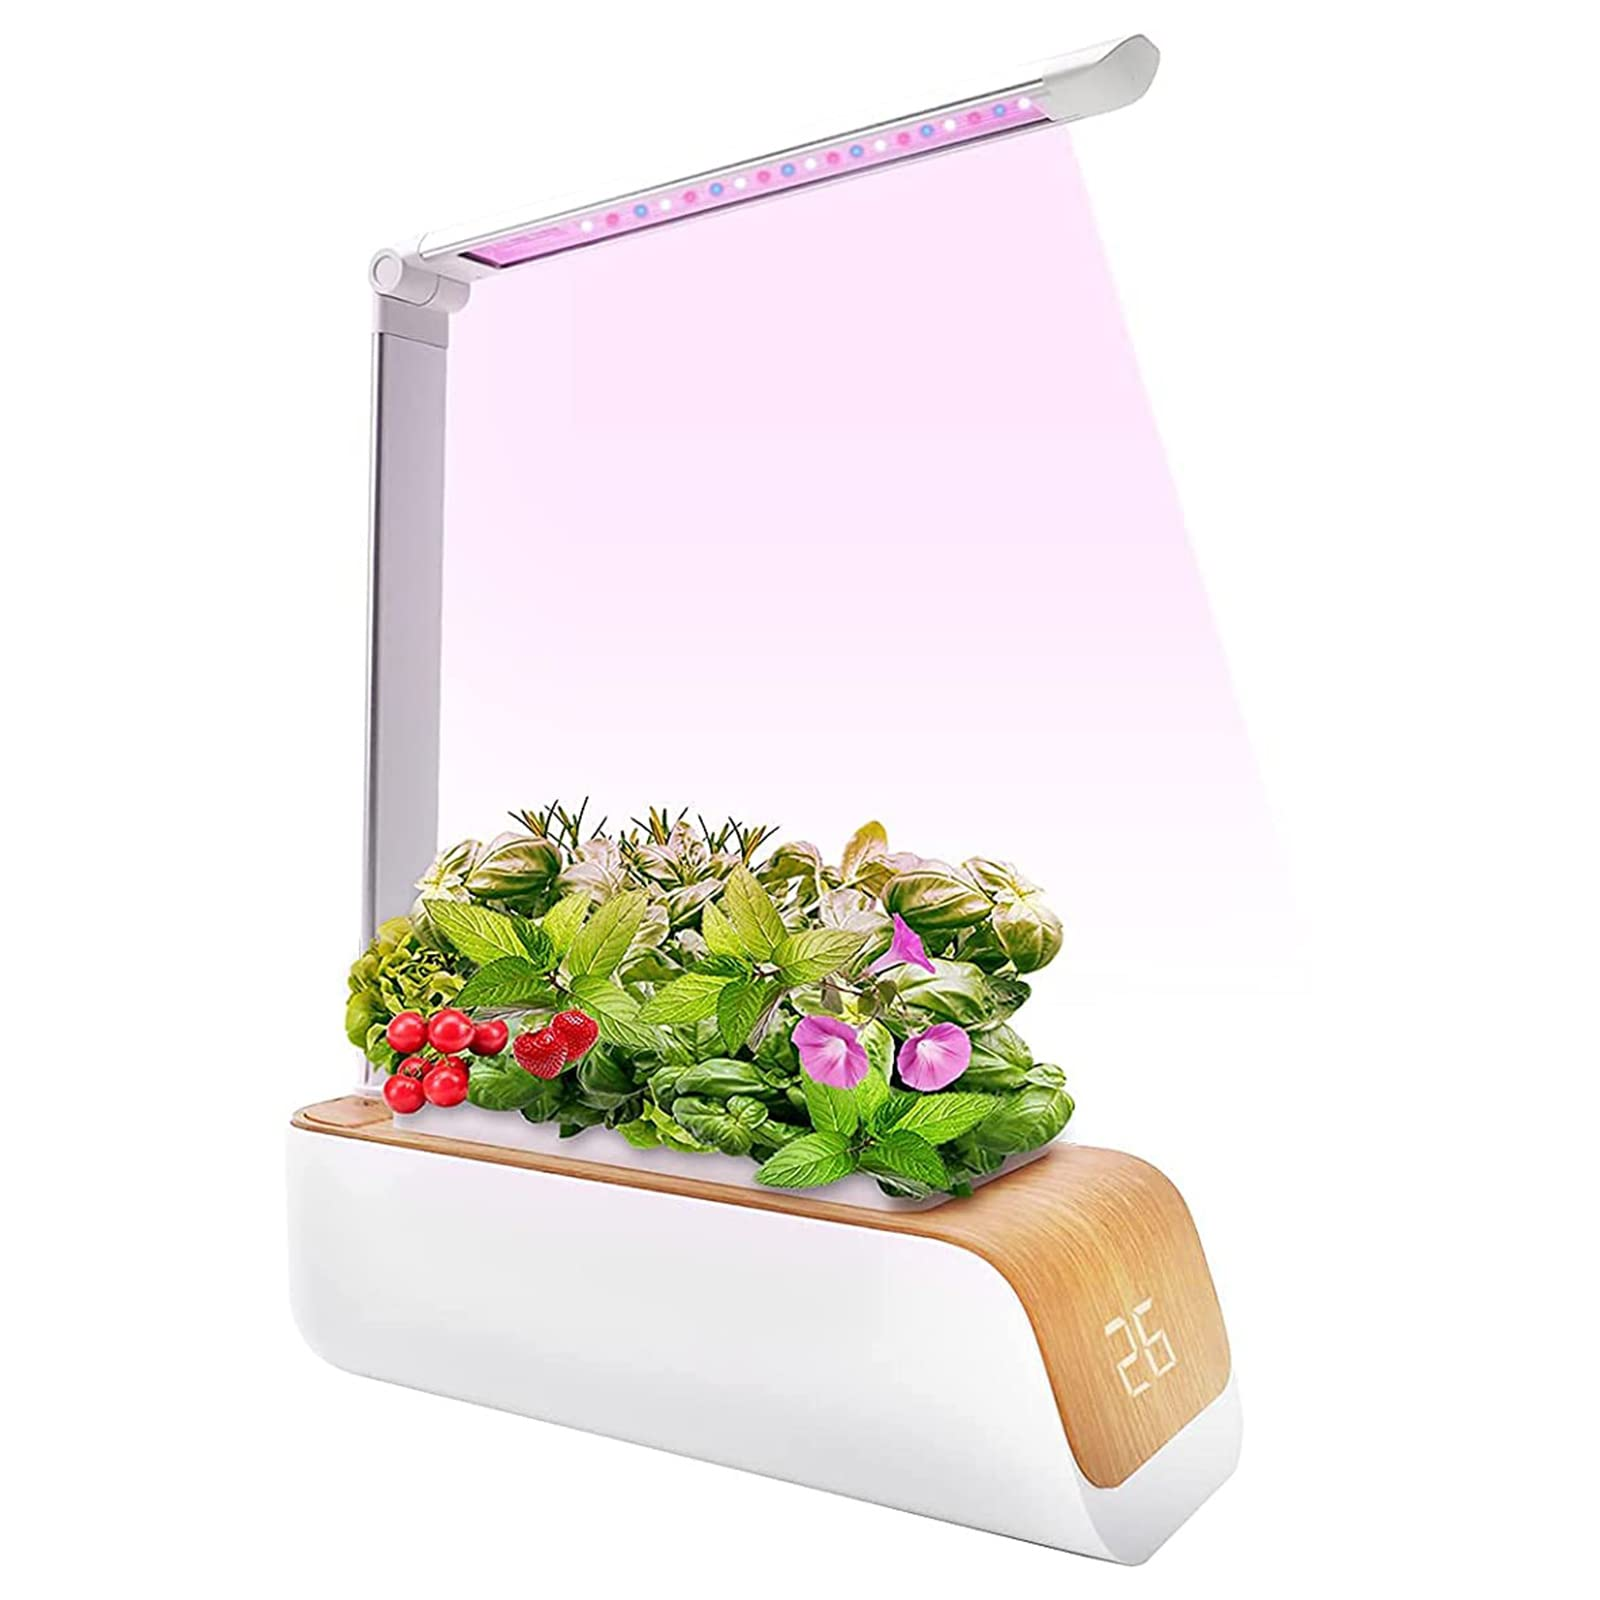
\includegraphics[width=0.5\textwidth]{images/hydro.jpg}
\caption{Ein Hydroponisches Anbausystem}\cite{zpyxbh_amazon}
\label{fig:hydro}
\end{figure}

Viele Produkte konzentrieren sich auf die Anzucht. Diese kosten zwischen 90 Euro \textcite{emsa_amazon} und 450 Euro \textcite{geberioz_amazon}. Sie nutzen überwiegend ein hydroponisches System, bei dem Pflanzen ohne Erde, lediglich durch einen konstanten, langsamen Wasserzufluss mit einer Nährstofflösung, aufgezogen werden. Diese Technik ist sehr effizient und ermöglicht eine genaue Kontrolle des Pflanzenwachstums.\textcite{pflanzenfabrik_tropfsystem} 

Die Geräte sind mit einem Wassertank und einem Platz für produktspezifische Pads ausgestattet, die die Pflanzen mit den richtigen Nährstoffen versorgen. Über Schläuche wird ein konstanter Wasserzufluss gewährleistet. Zusätzlich sind mehrere LED-Lampen angebracht, um den jungen Pflanzen ausreichend Licht zu geben, wobei auf Sonnenlicht meist nicht eingegangen wird. Diese Geräte erfordern normalerweise keine externe Steuerung, da Wasserzufluss und Licht vom Hersteller vorgegeben sind. Unterschiede zwischen den Pflanzen werden dabei nicht berücksichtigt. Hochpreisige Alternativen bieten manchmal eine Steuerung über Smartphone-Apps oder Fernbedienungen an, wobei Pumpe und Licht separat kontrolliert werden können, jedoch keine vollständig automatisierte Anpassung stattfindet.

Diese Systeme agieren automatisch und nicht intelligent.

\paragraph{Smart Vases}
\begin{figure}[H]
\centering
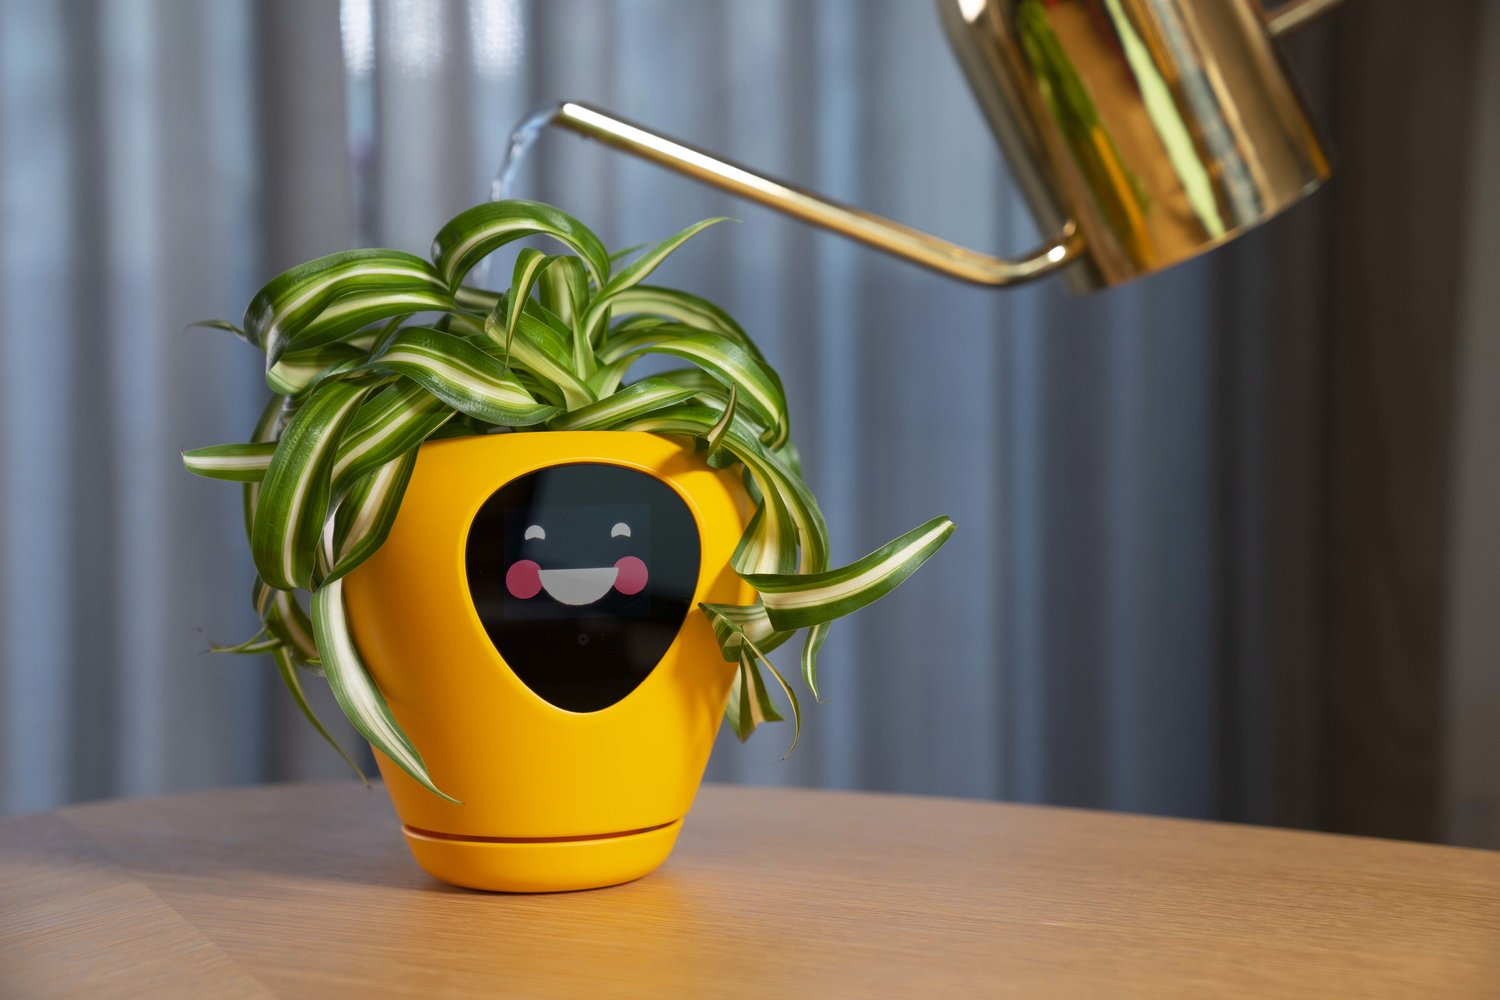
\includegraphics[width=0.5\textwidth]{images/Lua.jpg}
\caption{Eine Smart Vase mit Display}\cite{lua}
\label{fig:smartVase}
\end{figure}

Wesentlich geringer ist das Angebot bei Smarten Vasen. Diese kombinieren verschiedene Sensoren mit dem Verhalten eines digitalen Haustiers. Bei Kosten von etwa 150€\cite{lyeva_amazon} besitzen sie ein Display, auf dem die verschiedenen 'Gemütszustände' der Pflanze angezeigt werden. Über Emojis wird beispielsweise angezeigt, ob die Pflanze gegossen werden muss oder es an Sonnenlicht fehlt. Andere Produkte integrieren weitere 'Haustierfunktionen', wie ein Verlangen nach Aufmerksamkeit oder haptischer Berührung. Pflanzenpflege wird auf diese Weise gamifiziert\gls{Gamification} und durch das Display wird Aminismus erzeugt, das Zuschreiben von Persönlichkeit an ein lebloses Objekt. Die aufgebaute Beziehung sorgt für ein erhöhtes Verantwortungsbewusstsein\cite{lawton_tamagotchi_2017} und soll der Pflanzenpflege mehr Bedeutung geben, sowie die Nutzenden motivieren. 

Diese Maschinen besitzen in der Regel keine Aktoren; die Nutzenden müssen sich weiterhin selbst um die Pflanze kümmern. Zudem können sie nicht auf spezifische Pflanzen zugeschnitten werden, da die Richtwerte vom Hersteller vorgegeben und allgemein gehalten sind.

Diese Systeme gehören zu den intelligenten Systemen erster Art.

\paragraph{Automatische Bewässerungssysteme}
Im Freien existieren verschiedene Geräte zur Bewässerung von Pflanzen. Eine Sprenkleranlage wird automatisch durch eine kontinuierliche Wasserversorgung aktiviert, wodurch die Nutzenden keine manuelle Bedienung vornehmen müssen. Einige Geräte integrieren intelligente Funktionen. Durch einen WLAN-Adapter können Wettervorhersagen eingebunden werden, um das Bewässern bei Regen zu vermeiden oder durch Bodenfeuchtesensoren übermäßige Bewässerung zu verhindern und besonders sonnenintensive Tage auszugleichen. Zudem können mittels verschiedener Programme, häufig über Smartphone-Apps zugänglich, individuelle Bewässerungszeiten festgelegt werden, beispielsweise ausschließlich nachts statt tagsüber. Intelligente Varianten dieser Geräte tragen dazu bei, den Wasserverbrauch zu reduzieren. Die Preisspanne für derartige Produkte liegt zwischen ca. 70€ und 200€.\cite{rainpoint_smart_timer} 

Obwohl diese Maschinen primär für größere Gärten konzipiert sind, lässt sich ihr Ansatz auch auf die Intelligente Vase anwenden. Der Hersteller Rainpoint veranschaulicht die Funktionsweise dieses Geräts. Der Controller verbindet sich dabei mit der Cloud, auf die die Nutzenden über ihr Smartphone zugreifen können. Diese Geräte können entweder der Automatischen oder der Intelligenten Kategorie der 1. Art zugeordnet werden.

\begin{figure}[H]
\centering
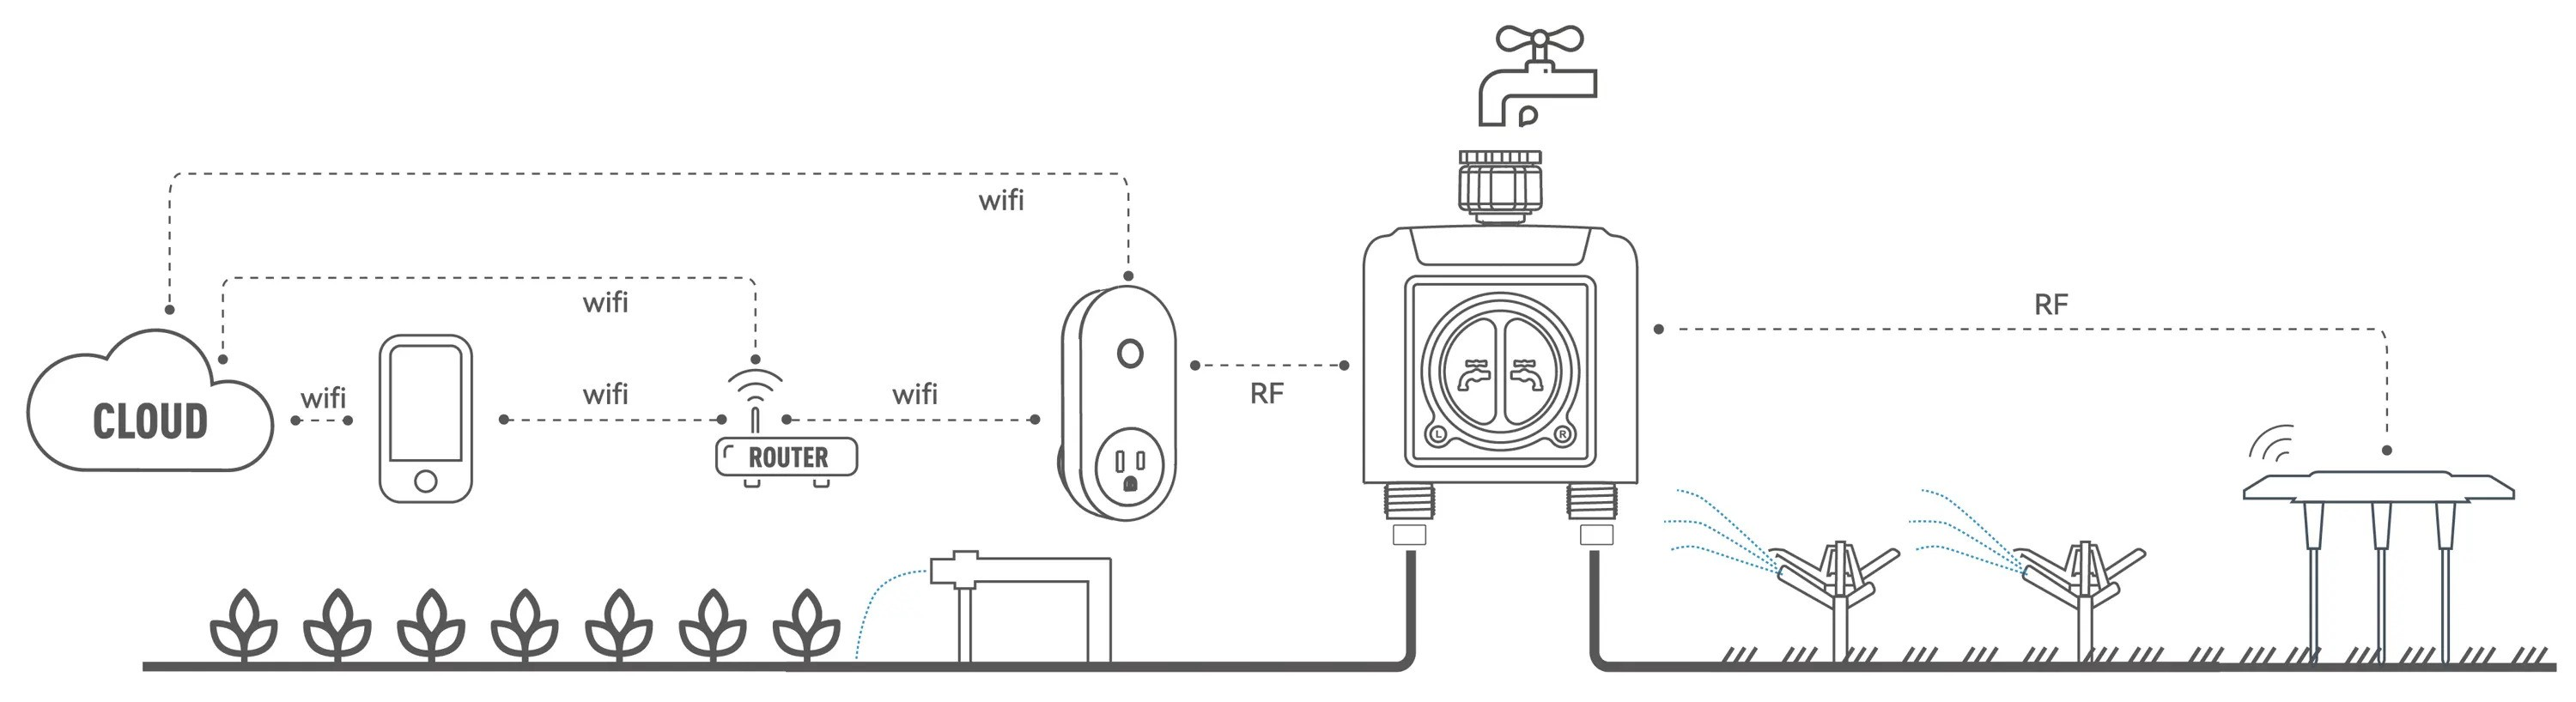
\includegraphics[width=\textwidth]{images/rainpoint.jpg}
\caption{Diagramm des Herstellers Rainpoint}\cite{rainpoint_smart_timer}
\label{fig:rainpointDiagram}
\end{figure}

Diese Geräte können zur automatischen oder zur intelligenten Kategorie der 1. Art zählen.

\subsection{Agrikulturelle Forschung}
"Die Landwirtschaft ist bis heute die wichtigste Erwerbsquelle und der größte Wirtschaftszweig der Welt. Ein Drittel aller arbeitenden Menschen ist in der Landwirtschaft beschäftigt."\cite{zukunftsstiftung_landwirtschaft}

Mit zunehmendem Bevölkerungswachstum und gesteigertem Konsum trägt die Landwirtschaft vier Prozent zum gesamten weltweiten Bruttoinlandsprodukt bei. Die Möglichkeit, durch Automatisierung Arbeitskräfte einzusparen, die Natur zu schonen und nachhaltig zu nutzen sowie profitablere Ernten zu erreichen, hätte einen erheblichen globalen Einfluss. Die Europäische Kommission betrachtet Innovation und Fortschritt als eine ihrer wichtigsten Aufgaben in den kommenden Jahren .\cite{eu_agriculture}

Ein großer Fokus der agrarischen Automatisierung liegt auf der Bewässerung. Mithilfe verschiedener Algorithmen und KI-Modelle wird versucht, Wasser möglichst effizient einzusetzen und Verschwendung zu vermeiden. Die Grundlage für eine automatische Bewässerung besteht aus drei Schritten:\cite{kumar2018automatic}

\begin{itemize}
    \item Aufnahme der Bodenfeuchtigkeit mittels Sensoren
    \item Vergleich mit internen Datenbanken bezüglich des optimalen Feuchtigkeitswerts
    \item Reaktion durch Ein- oder Ausschalten der Pumpe
\end{itemize}

Wahlweise können Daten auch für weitere Forschungszwecke gespeichert werden. In größeren Anbaugebieten, in denen nicht jeder Quadratmeter vermessen werden kann und verschiedene Pflanzen angebaut werden sowie komplexere Pumpsysteme eingesetzt werden, können auch komplexere Systeme wie Fuzzy-Controller verwendet werden, um die gesamte Fläche effektiv zu bewässern .\cite{mushtaq2016automatic}

Gewächshäuser ermöglichen den Anbau kälteempfindlicher Pflanzen auch in kalten Regionen. In den meisten Konzepten kann erwärmte Luft von Sonnenstrahlen nicht nach außen entweichen, was die Temperatur innerhalb des Gewächshauses erhöht. Um optimales Pflanzenwachstum zu gewährleisten, darf die Temperatur jedoch nicht zu hoch sein. Verdunstungskälte, Ventilatoren oder Raumöffnungen können hier Abhilfe schaffen. Auch hier werden seit Langem automatisierte Verfahren verwendet. Das Grundprinzip ähnelt dem der Bewässerung:\cite{seesansui2020automatic}

\begin{itemize}
    \item Aufnahme der Lufttemperatur mittels Sensoren
    \item Vergleich mit internen Datenbanken bezüglich des optimalen Temperaturwerts
    \item Reaktion durch Ein- oder Ausschalten der Kühlungsmethoden
\end{itemize}
Auch hier könnten sich Fuzzy-Controller eignen, falls mehrere Möglichkeiten zur Kühlung existieren. Oft wird die Temperaturregelung in Gewächshäusern mit automatischer Bewässerung kombiniert.\cite{al-humairi2019smart}

Inzwischen werden auch komplexere Machine Learning Techniken verwendet, um Pflanzen optimal zu überwachen.

\paragraph{Integration von Machine Learning Systemen in der Champignon Zucht\cite{barauskas2022approach}}
In einer Champignon-Zucht in Litauen wurde über die letzten Jahre ein Klimamanagementsystem entwickelt. Dabei sammelten Umweltsensoren Daten wie die Komposttemperatur, Luftfeuchtigkeit, CO²-Gehalt in der Luft und weitere Informationen während der verschiedenen Wachstumsphasen der Pilze. Diese Informationen wurden über eine Benutzeroberfläche ausgegeben und konnten verschiedene Werte anhand vorgegebener Richtlinien anpassen (intelligentes System zweiter Art). Forschende kamen nun auf die Idee, ein System zu integrieren, das anhand des aktuellen Zustands der Pilze Empfehlungen für Veränderungen gibt. Das Modell verknüpft hierbei Umweltdaten mit visuellen Informationen. Verschiedene Kameras nehmen in regelmäßigen zehnminütigen Abständen Fotos vom Zustand der Zucht auf. Erkennt der Computer Verbesserungsmöglichkeiten, werden diese dem Team mitgeteilt.

\begin{figure}[H]
\centering
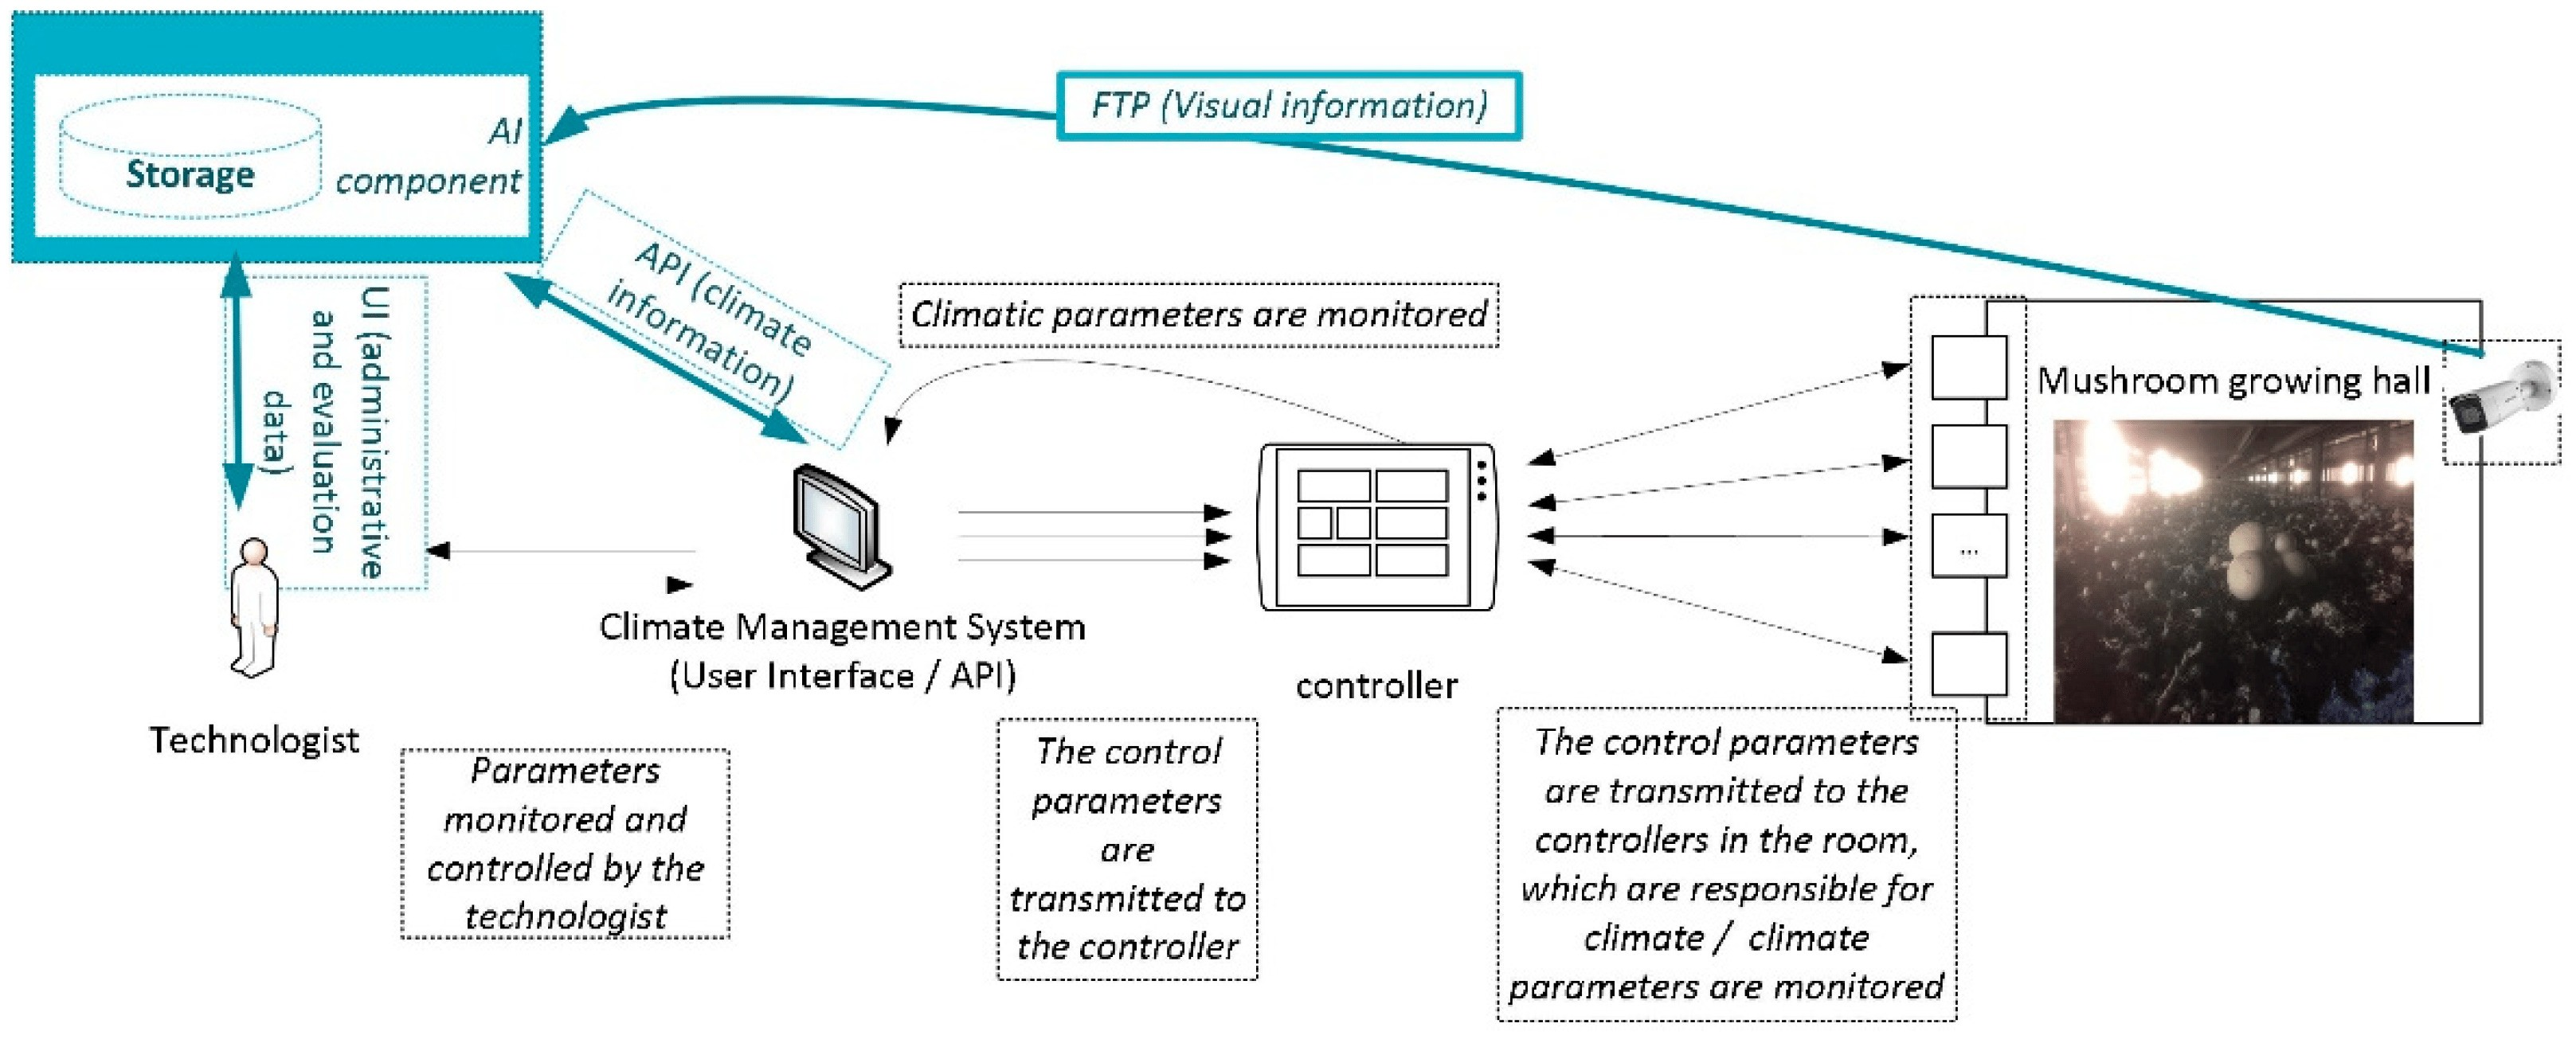
\includegraphics[width=\textwidth]{images/mushroom.jpg}
\caption{Diagramm der AI-Einbindung in der Champignon Aufzucht}\cite{rainpoint_smart_timer}\cite{barauskas2022approach}
\label{fig:mushroomDiagramm}
\end{figure}

Das Projekt bietet Einblicke, wie verschiedene KI-Tools in die Pflanzenaufzucht integriert werden können. Es werden auch die genauen Technologien beschrieben. So wurden aufgenommene Bilder nicht nur auf die Größe der Pilze untersucht, sondern auch die des Myzels, der fädenförmigen Zellen eines Pilzes. Zur genaueren Analyse wurde die Fourier-Analyse genutzt. Dabei werden komplexe Signale in einzelne Sinus- und Kosinuswellen aufgespalten und unerwünschtes Rauschen entfernt, um Muster zu erkennen.\cite{fourier_transformation} Hier wurden drei verschiedene schwarz-weiß Bilder (a, e, i) verwendet, die innerhalb von 8 Tagen aufgenommen wurden. Diese Bilder wurden durch drei verschiedene Filter analysiert, die jeweils tiefe (b, f, j), mittlere (c, g, k) und hohe Frequenzen (d, h, l) zulassen. Tiefe Frequenzen stehen hierbei für graduelle Unterschiede in der Farbe, beispielsweise den verschiedenen Weißtönen des Pilzes, während hohe für starke Kontraste stehen, wie etwa die Kante zwischen Pilz und Boden.

\begin{figure}[H]
\centering
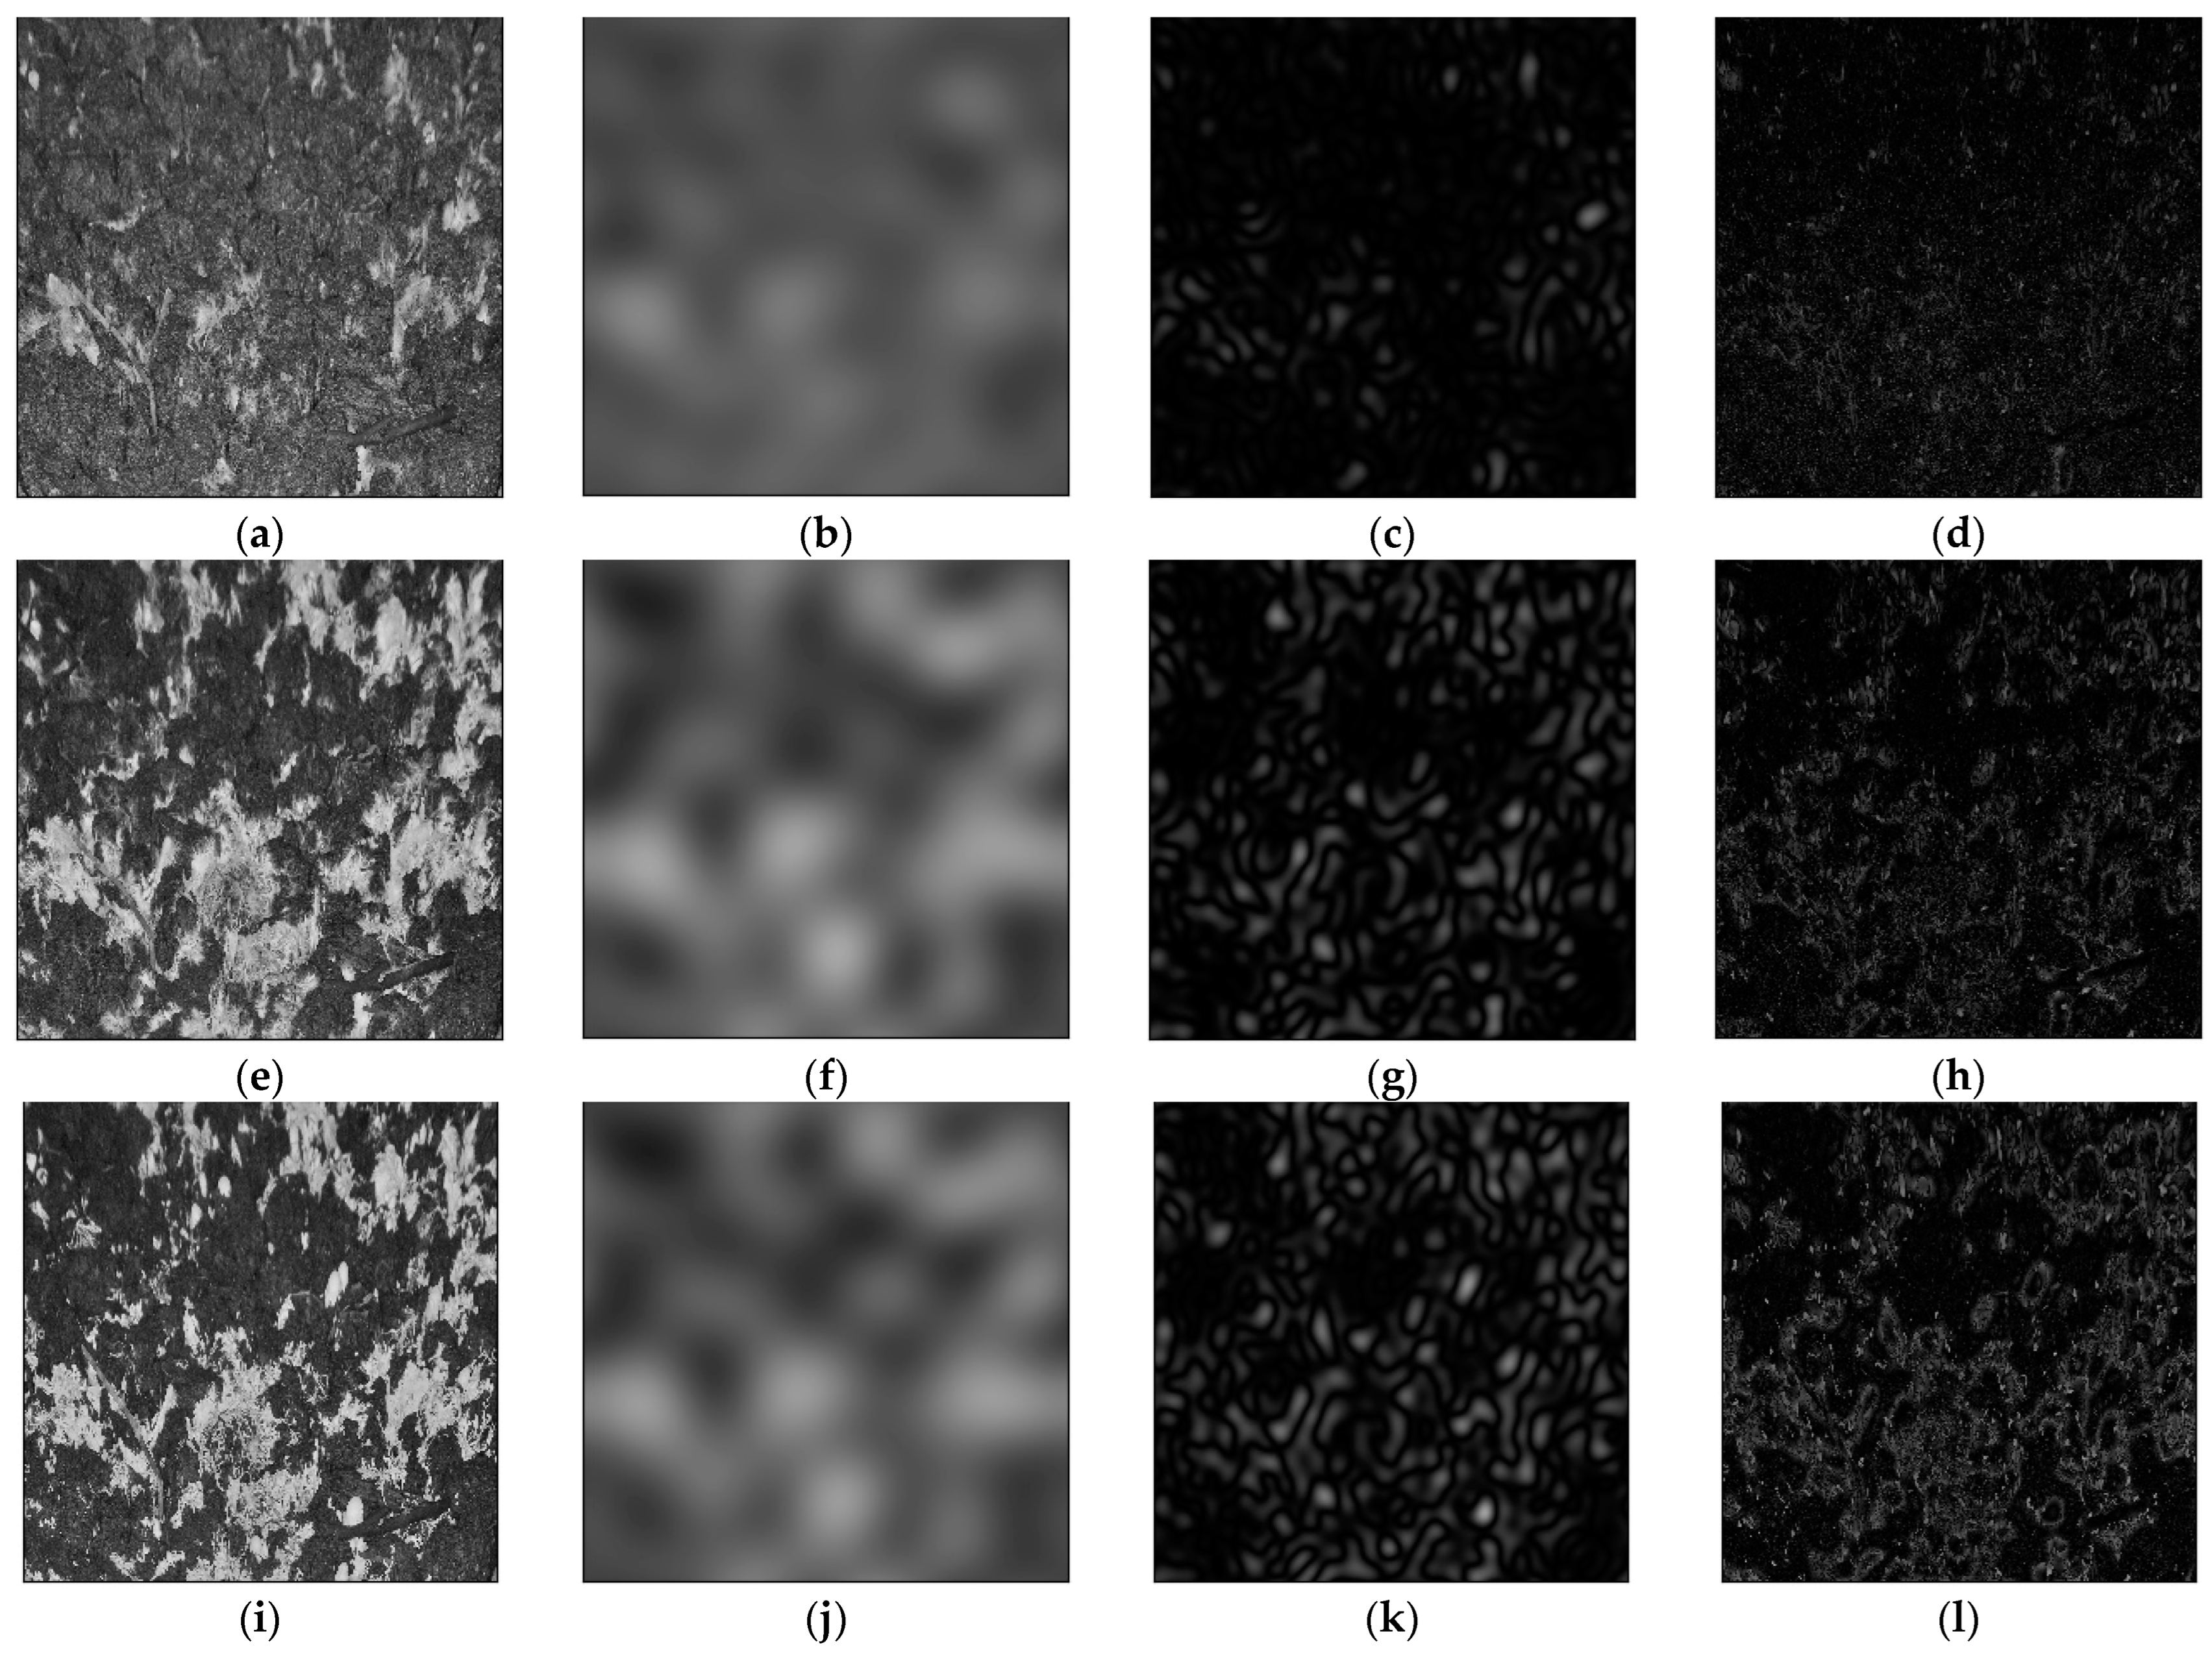
\includegraphics[width=\textwidth]{images/mushroomFreq.png}
\caption{Bildverarbeitung anhand der Fourier Analyse}\cite{rainpoint_smart_timer}\cite{barauskas2022approach}
\label{fig:mushroomDiagramm}
\end{figure}

Mithilfe der Morphologischen Analyse\gls{MorphA} kann erkannt werden, wie viele einzelne Myzel-Flächen existieren und wie groß diese sind. Um die einzelnen Pilze zu erkennen, wurde das Faster R-CNN (Region-based Convolutional Neural Network) Verfahren verwendet. Regions of Interest (ROI), für den Computer relevante Abschnitte, werden hierbei erkannt, mithilfe von Selective Search\gls{SelecSea} und einem Greedy Algorithmus\gls{Greedy Algorithmus} zu maximal 2000 Objekten zusammengefasst und mit Rechtecken umrandet.\cite{object_detection_algorithms} Anschließend werden die ROIs durch ein Neuronales Netzwerk analysiert, um den Objekttyp zu bestimmen. Beim Faster R-CNN wird die Auswahl der Regions of Interest in das Neuronale Netzwerk integriert, was den Vorgang deutlich beschleunigt. Mithilfe von realen Markern, die in den Boden gesetzt wurden, konnten die Maße der Objekte in reale Daten umgesetzt und in verschiedene Kategorien gefasst werden.

Für eine sorgfältige Bildanalyse sollten also in jedem Fall verschiedene Bilder über mehrere Tage hinweg verwendet werden. Diese werden unterschiedlich aufbereitet, um möglichst vielfältige Informationen zu bieten, damit das System das gewünschte System möglichst genau erkennen kann.

Die über mehrere Wochen gesammelten Daten konnten benutzt werden, um das Wachstum und die Gesundheit der Pilze unter verschiedenen Umweltbedingungen in den verschiedenen Wachstumsphasen einzuschätzen. Mit diesen Daten konnten Algorithmen entwickelt werden, um Empfehlungen für das Team bezüglich des Pflanzenwachstums zu geben.

Die Entscheidungsfindung basiert auf einem Entscheidungsbaum\gls{Entscheidungsbaum}. Es werden sowohl Expertenmeinungen, die visuellen Daten als auch die Klimaparameter berücksichtigt. Die Merkmale werden in 4, 12 und 24 Stunden Intervallen betrachtet. Die Werte werden mit den am ähnlichsten vergangenen Versuchen verglichen. Daraus wird abgeleitet, ob eine Änderung der Parameter erforderlich ist. Ist dies der Fall, werden die Werte mit der besten Wachstumsprognose empfohlen. Hierbei wird das Prinzip des K-nearest-neighbors (KNN) verwendet. Über den gesamten Ablauf muss permanent geprüft werden, ob die Eingangsdaten korrekt sind und der Entscheidungsbaum anhand der Daten eine sinnvolle Empfehlung geben kann. Ist dies nicht der Fall, wird der Automationsprozess abgebrochen. Es benötigt also einige Züchtungen, bis dem System genügend Daten zur Verfügung stehen und es sinnvolle Empfehlungen geben kann.

\begin{figure}[H]
\centering
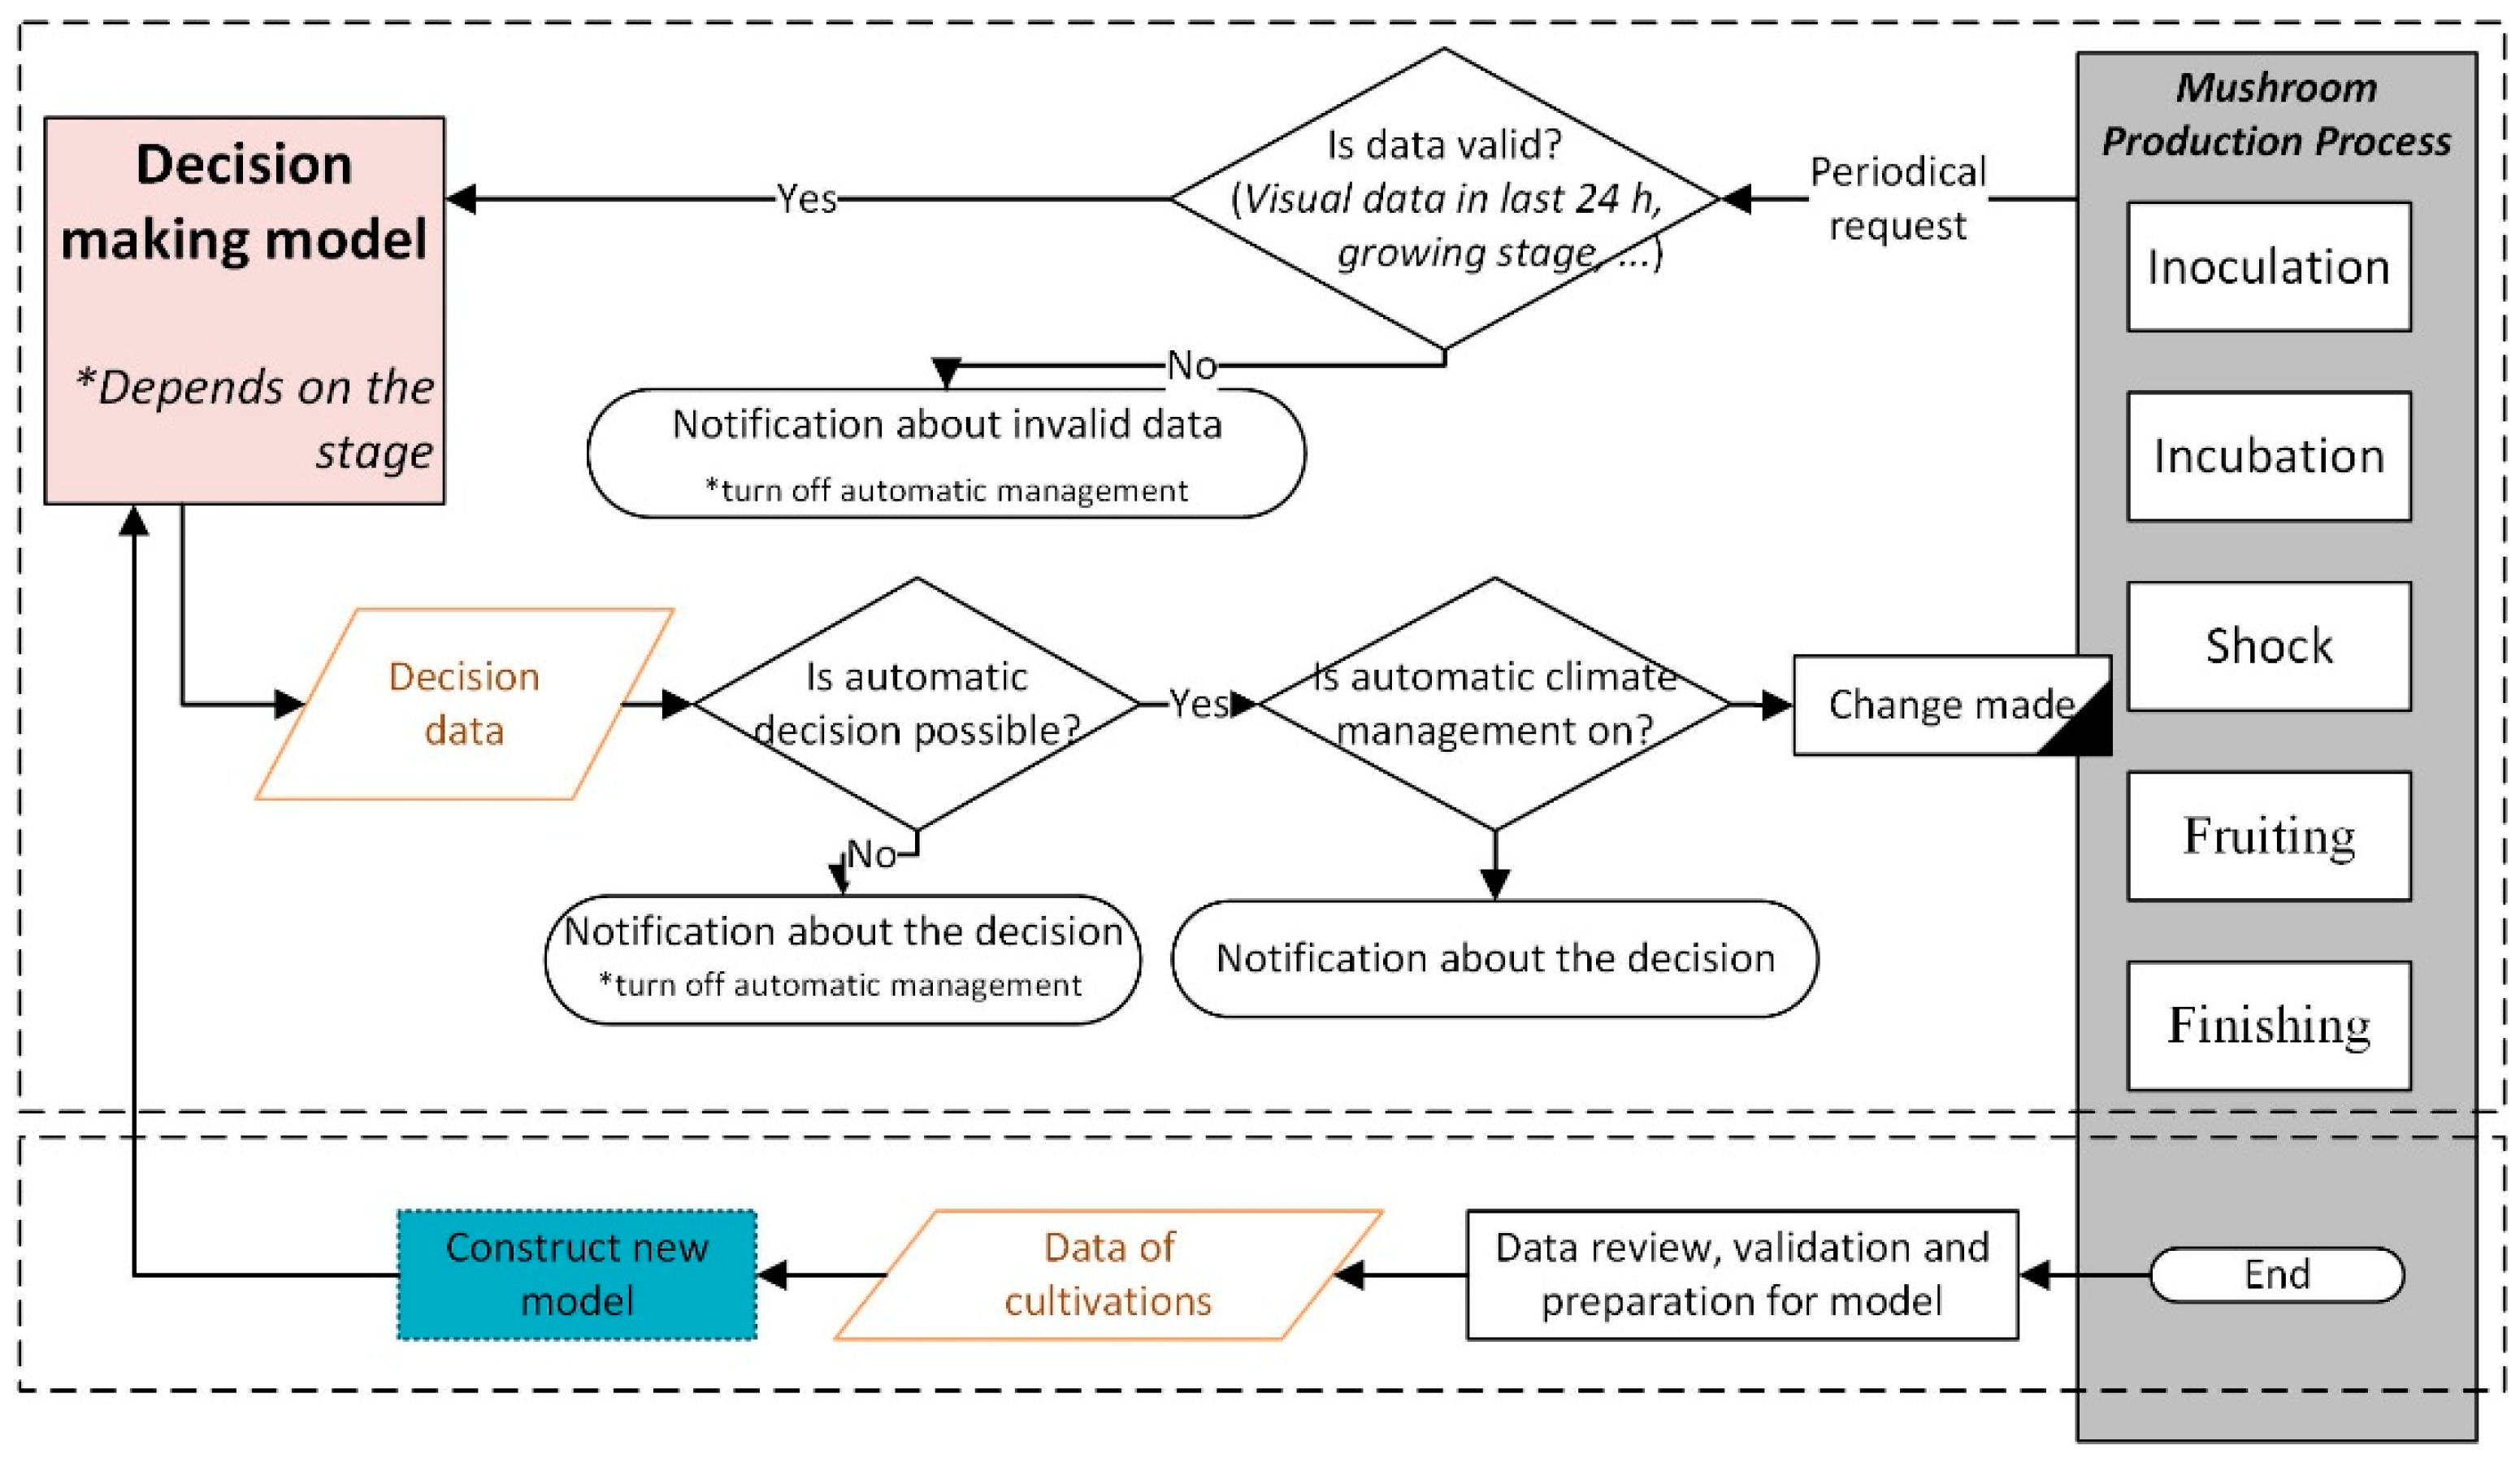
\includegraphics[width=\textwidth]{images/decisionTree.png}
\caption{Prozess der Entscheidungsfindung\cite{barauskas2022approach}}
\label{fig:mushroomDiagramm}
\end{figure}

Obwohl die Studie mit einer geringen Anzahl von Testdaten arbeiten musste, waren die Ergebnisse erfolgsversprechend. Der Algorithmus konnte mit überwiegender Sicherheit bestimmen, in welcher Wachstumsphase sich die Pilze befinden und ob eine Änderung des Klimas notwendig ist. Mit einem erhöhten Datensatz werden dann auch die empfohlenen Änderungen immer sicherer.

\paragraph{Werkzeuge in der Automation von Landwirtschaft mittels AI}\cite{jha2019comprehensive}
Experten Systeme wurden bereits seit den 80er Jahren in der Landwirtschaft eingesetzt. Basierend auf dem Fachwissen und den Meinungen von Expertinnen und Experten sollen diese Systeme Farmerinnen und Farmern bei allen Teilen des Anbaus unterstützen und wichtige Informationen liefern. Diese Systeme laufen meist nicht eigenständig und benötigen Input sowie die Einschätzung der Landwirtinnen und Landwirte, um genutzt werden zu können.

In einem Journal des Verlags KeAi fassten verschiedene Forschende aus Indien mögliche Anwendungen von KI in der Landwirtschaft zusammen . Künstliche neuronale Netzwerke\gls{ANN} sind hierbei die bekanntesten und werden für verschiedene Zwecke genutzt. ANN's benötigen zwar viele Daten, können jedoch aus diesen zu großen Teilen ihre eigenen Schlüsse ziehen. So können Zusammenhänge und Denkweisen erkannt werden, die bisher nicht berücksichtigt wurden. Zudem können sie mit weiteren Daten trainiert werden. Der Output bleibt nicht konstant und kann mit dem System wachsen, ohne weitere Programmierarbeit aufzuwenden. So kann beispielsweise der Reifegrad von Getreide, Pflanzenerkennung oder die Verfügbarkeit von Wasser eingeschätzt werden. In einer Studie zur Abschätzung der Maisernte wurden Multilayered Feedforward ANN's und einem Conjugate Gradient Descent Algorithm zur Gewichtung der Verbindungen verwendet.\cite{singh2008artificial} Fuzzy Logic \gls{Fuzzy Logic} hingegen wurde bei der Verbesserung eines Expertensystems für Sojabohnen eingesetzt. Da viele Werte wie Pestbefall oder Bodenqualität nicht einfach als binärer Wert ausgegeben werden können, wurde sich hier für einen Fuzzy-Logik-Ansatz entschieden.\cite{prakash2013fuzzy}

Oft werden dabei sogenannte positivistische und systematische Methoden kombiniert. Positivistische Methoden sind eher "hands-on", und die Algorithmen funktionieren ähnlich wie das Vorgehen von Expertinnen und Experten. Bei systematischen Methoden hingegen ist das System mehr auf sich allein gestellt und soll eigene Wege finden, um Ergebnisse zu erzielen. Eine einzelne Methode ist in manchen Fällen ineffizient oder nicht genau genug. In solchen Fällen kann eine Kombination sinnvoll sein, um alle wichtigen Bereiche abzudecken.

\paragraph{Zusammenfassung}
Die verschiedenen Produkte und Studien zeigen, dass Automatisierungsprozesse in der Pflanzenpflege bereits jetzt von immenser Bedeutung sind und unter der Überwachung von Expertinnen und Experten den Prozess vereinfachen und bessere Ergebnisse erzielen können. Sensoren, regelbasierte Systeme, Fuzzy-Logik, Künstliche neuronale Netzwerke (ANN's), Mustererkennung und Bildverarbeitung/Maschinenvision werden alle im Bereich der Landwirtschaft eingesetzt, oft in Kombination. Bei der Entwicklung eines neuen Produkts kann auf eine Vielzahl von Werkzeugen und Technologien zurückgegriffen werden, um das gewünschte Ergebnis zu erzielen. Diese bereits implementierten Technologien können zu großen Teilen auch im privaten Bereich eingesetzt werden, um die Pflanzenpflege zu erleichtern.

\subsection{Theoretische Grundlage des Machine Learning\gls{Machine Learning} Verfahrens}
Im vorangegangenen Abschnitt wurde aufgezeigt, dass viele verschiedene algorithmische Verfahren verwendet werden, um die Pflanzenpflege zu automatisieren. In diesem Abschnitt wird genauer beleuchtet, wie diese Verfahren funktionieren und in welchen Anwendungsgebieten sie eingesetzt werden sollten.

Generell wird zwischen überwachtem (Supervised) und unüberwachtem (Unsupervised) Lernen unterschieden. Überwachtes Lernen bedeutet hierbei, dass ein Mensch manuell Ergebnisse überprüft und eine Richtung vorgibt, während beim unüberwachten Lernen der Algorithmus vollkommen eigenständig seine Ergebnisse erzielt. Bei komplexen Projekten wie diesem ist es von Vorteil, Technologien aus beiden Arten zu kombinieren, um sowohl Expertenwissen als auch maschinelle Erkenntnisse zu vereinen.

Im Folgenden werden drei verschiedene Machine-Learning-Ansätze vorgestellt. Alle können bei der Entscheidungsfindung in der Pflanzenpflege hilfreich sein und können unterschiedlich kombiniert werden, um bestmögliche Ergebnisse zu erzielen.

\paragraph{Fuzzy Logic}
Über den verschiedenen Methoden steht die Entscheidung, ob Fuzzy- oder Boolesche Logik verwendet werden sollte. Anders als bei Booleschen Entscheidungen ermöglichen Fuzzy-Logic-Algorithmen eine Entscheidung bei ungenauen Werten. Numerische Zustände wie 21 Grad Celsius können in linguistische Zustände (Sets) wie "kalt" oder "warm" umgewandelt werden.\cite{lameres1998fuzzy} Reale Szenarien, bei denen menschliche Einschätzungen benötigt werden, können so wesentlich besser behandelt werden.

Fuzzy Logic basiert immer auf einer Architektur mit vier Teilen.\cite{fuzzy-logic-introduction} Um es deutlicher zu machen, wird der Ablauf anhand einer automatischen Klimaanlage aufgezeigt:
\begin{enumerate}
    \item Im Regelwerk werden alle Abläufe von Expertinnen und Experten festgesetzt. Im Normalfall werden Fälle in "stark positiv", "positiv", "neutral", "negativ" und "stark negativ" eingeteilt. Ist es sehr heiß, schalte die Klimaanlage auf maximale Leistung an. Ist es nur warm, reicht eine geringere Leistung. Ist es zu kalt, schalte die Heizung an.
    \item Während der Fuzzification werden aus den eindeutigen Inputs, wie der gemessenen Gradanzahl, unscharfe Mengen gebildet. So wird beispielsweise alles zwischen drei und zehn Grad als "moderat kalt" eingestuft.
    \item Die Inferenzmaschine ordnet den unsicheren Input einer Regel zu. Wenn es warm ist, schalte die Klimaanlage auf moderater Leistung an.
    \item Während der Defuzzification wird die unsichere Menge und die Regel zu einem klaren Wert konvertiert. Die Klimaanlage wird mit 65 Prozent Leistung angeschaltet. Da verschiedene Inputs zu Sets zusammengefasst werden, ist ein Informationsverlust unvermeidbar.
\end{enumerate}

Fuzzy Logic ist um einiges flexibler als gewöhnliche Entscheidungsbäume und ist gut geeignet, um menschliches Handeln umzusetzen. Verschiedene numerische Variablen können zu Sets verbunden werden, um ein komplexes Regelwerk zu erstellen. Bei den Inputs "Spannung" und die "Schnelligkeit der Änderungsrate der Spannung", beispielsweise NM für "Negative Medium" und PL für "Positive Large", kann das Regelwerk für den Output der Spannung folgendermaßen aussehen:

\begin{figure}[H]
\centering
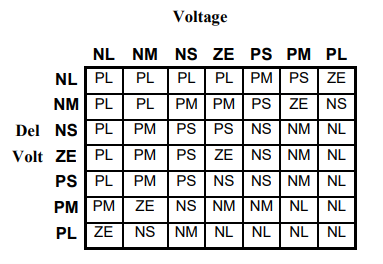
\includegraphics[width=\textwidth]{images/fuzzyVolt.png}
\caption{Regelwerk für eine Spannungsausgabe. \cite{lameres1998fuzzy}}
\label{fig:Fuzzy Voltage Controller}
\end{figure}

Ergebnisse sind hierbei nicht zwingend optimal, aber ausreichend, und es ist einfacher, mit komplexen Situationen umzugehen. Fuzzy Logic sollte nicht benutzt werden, wenn die Ergebnisse exakt sein müssen. Auch dauern die Berechnungen im Vergleich zu anderen Machine-Learning-Algorithmen lange.

\subsubsection{}{Decision Tree}
Decision Trees sind eines der einfachsten zu implementierenden Machine-Learning-Verfahren. Sie gehören zu den überwachten Lernalgorithmen, bei denen Daten vom Ersteller gelabelt werden, und die Maschine trifft keine eigenen Einschätzungen darüber, was richtig und falsch ist. Diese Methode kann sowohl für klassifizierte als auch für regressionsbasierte Aufgaben verwendet werden.

Wenn wir beispielsweise vorhersagen möchten, ob eine Pflanze wachsen wird, sind verschiedene Daten wichtig: Temperatur, Bodenqualität, Sonneneinstrahlung, Wasserzufuhr, etc. Alle diese Daten bilden den Root-Node, der dann gesplittet wird. Hierbei wählt der Algorithmus eine Eigenschaft aus, die den Datensatz am eindeutigsten teilt. Während einige Pflanzen auch bei niedrigen Temperaturen wachsen können, kann keine Pflanze ohne Wasserzufuhr wachsen. Diese Variable teilt den Datensatz in Sub-Nodes auf. Wenn diese Nodes weiter unterteilt werden können, bezeichnet man sie als Entscheidungs-Nodes, sonst als Blatt-Nodes. Sind bestimmte Eigenschaften nicht relevant, werden sie vom Algorithmus entfernt, das sogenannte "Pruning". So entstehen Branches, die die Entscheidung des Systems bestimmen.

Decision Trees können bei großen Datensätzen sehr komplex werden und den Hintergrundrauschen (nicht relevante Eigenschaften) nicht von den relevanten Mustern unterscheiden. Techniken wie Pruning und die Begrenzung der Tiefe können hierbei helfen. Auch können kleine Änderungen des Datensatzes zu gänzlich anderen Bäumen führen. Die Herausforderung besteht darin, die entscheidenden Attribute zu filtern, sodass nicht für jeden Fall des Trainingssets ein Blatt-Node gebildet wird, sondern das System andere Daten sinnvoll einschätzen kann.

Wann ein Node in welche Subnodes gesplittet wird, ist der wichtigste Entscheidungsfaktor für die Effektivität des Algorithmus. Das System muss hierbei entscheiden, welche Attribute eine hohe Entropie aufweisen, das Ergebnis zufällig beeinflussen, und aus welchen man einen hohen Informationsgewinn erlangen kann, um den Datensatz möglichst homogen zu splitten.\cite{decision-tree-explained} Diese Einschätzung muss von einem Experten vorgenommen werden. Dabei gibt es verschiedene Algorithmen, die je nach Anwendung unterschieden werden sollten, unter anderem:

\begin{itemize}
    \item ID3: Der Algorithmus entscheidet bei jeder Iteration, welches Attribut die niedrigste Entropie und den höchsten Informationsgewinn hat, und bildet darauf ein Subset.
    \item C4.5: Hier wird der normalisierte Informationsgewinn verwendet und über die Entropie gestellt.
    \item CART: Ein Decision Tree, der für die Klassifikation optimiert ist.
    \item MARS: Ein Decision Tree, der für die Regression optimiert ist.
\end{itemize}

\subsubsection{Artificial Neural Networks}
Das menschliche Gehirn filtert aus einer schier unendlichen Masse an Informationen mit geringem Aufwand unwichtige Informationen heraus und führt schnelle Berechnungen durch. Dies geschieht durch einen scheinbar simplen Vorgang, bei dem Rezeptoren Signale an Effektoren senden und diese Informationen weiterleiten. Diese Einheiten werden als Neuronen bezeichnet. Wenn dieselben Wege immer wieder benutzt werden, wächst das Netzwerk an Verbindungen und wird effektiver.\cite{stiftung2023nervensystem}

Künstliche neuronale Netze sind stark vom menschlichen Gehirn inspiriert und sollen aus großen und komplexen Datenmengen sinnvolle Ergebnisse erzielen. Dies geschieht in drei Schichten:\cite{wuttke2023neuronale}

\begin{itemize}
    \item Eingabeschicht: Hier werden die eingegebenen Daten aufgenommen und an die richtigen Eingabeneuronen weitergeleitet. Diese gewichten die Eingaben und geben sie an die nächste Schicht, bestehend aus einem oder mehreren Neuronen, weiter.
    \item Verborgene Schicht: Diese Schicht kann aus beliebig vielen Ebenen bestehen. Die angenommene Information wird hier beliebig oft weitergewichtet und weitergeleitet.
    \item Ausgabeschicht: Dies ist die letzte Schicht. Die gewichtete Information wird gespeichert und ausgegeben.
\end{itemize}

Ein Neuron sammelt die Informationen aller vorangegangenen Neuronen, mit denen es verbunden ist, und multipliziert diese anhand der Gewichtung. Dann wird dieser Wert durch eine Aktivierungsfunktion auf einen Wert zwischen Null und Eins normalisiert.\cite{arnx2019first}

Die Gewichtung wird zunächst zufällig verteilt. Wenn sie den richtigen Output generiert, bleibt die Gewichtung bestehen, wenn nicht, wird sie angepasst. Es gibt verschiedene Möglichkeiten, dem System zu sagen, ob der generierte Output korrekt ist:\cite{dongare2012introduction}

\begin{itemize}
    \item Beim Supervised Learning werden für jedes Beispiel die korrekten Output-Daten vorgegeben. Jede Mail im Trainingsset wird beispielsweise als Spam oder Nicht-Spam gekennzeichnet. Das System kann so erkennen, ob es die richtigen Indizes zur Erkennung verwendet.
    \item Beim Unsupervised Learning ist der Output oft vage und zu komplex zu beschreiben. Das System gruppiert die Daten selbst und erstellt Zusammenhänge. Beim Clustering werden Daten beispielsweise in Gruppen geordnet, um unbemerkte Muster zu erkennen.\cite{altexsoft2021unsupervised} Diese Methode wird oft für Empfehlungen in Online-Shops verwendet, um unbeachtete Patterns zu nutzen oder in Data Science, um Forschern zu helfen neue Zusammenhänge zu erkennen.
    \item Das Reinforcement Learning liegt zwischen den beiden Varianten. Das System erhält Informationen darüber, ob der Output zielführend war oder nicht. \cite{synopsys2024reinforcement} Mit jedem Trainingsdurchlauf soll die KI so besser werden. Bei einem Rennspiel entscheiden Gas und Lenkradrichtung über den Spielverlauf. Kann das Fahrzeug schneller ans Ziel gelangen, hat es die richtigen Vebindungen geschaffen. Die Reward-Funktion, welche Parameter belohnt werden und wünschenswert sind, kann über den Verlauf des Trainings verändert werden, um bestimmtes Verhalten zu fördern. Ähnlich wie ein Tennistrainer, der zur Aufgabe gibt lediglich Rückhand-Schläge zu üben, verliert auch die AI einmal erlerntes Wissen nur langsam und kann so neue Techniken lernen, im Realfall sehen, wann diese hilfreich sind, und so gezielt einsetzen.
\end{itemize}


ChatGPT
Das Konzept der Generalisierung ist von entscheidender Bedeutung in der künstlichen Intelligenz. Ähnlich wie ein Mensch kann eine KI bessere Ergebnisse erzielen, wenn der Rahmen enger gesteckt ist. Eine KI, die beispielsweise nur Bilder von Hunden in einem bestimmten Album erkennen soll (das Trainingsset)\gls{Trainingsset},wird dieses Ziel verhältnismäßig schnell und zuverlässig erreichen. Wenn jedoch das Ziel darin besteht, auf zufälligen Bildern Hunde zu erkennen, ist eine andere Gewichtung und ein breiterer Rahmen nötig. Die erstgenannte KI wird zwar im Trainingsset nahezu perfekt sein, aber in anderen Situationen kaum zu gebrauchen sein. Eine eher auf Generalisierung fokussierte KI wird generell gute Ergebnisse liefern, aber nie so genau wie die spezialisierte im Trainingsset. Hier liegt es am Entwickler, den richtigen Grad an Generalisierung zu wählen, um die gewünschten Ergebnisse zu erzielen.\cite{lark2023generalization}

Es gibt viele verschiedene Formen von Künstlichen Neuronalen Netzen, und je nach Anwendung muss die Art und die genaue Implementierung spezifiziert werden, um optimale Ergebnisse zu erzielen. Künstliche Neuronale Netze sollten verwendet werden, wenn die Trainingsdaten zu komplex sind oder die Datenstruktur nicht vollständig verstanden wurde. Sie bilden die Grundlage für viele weitere komplexe KI-Technologien.

\subsubsection{Pattern Recognition}
Pattern Recognition ist eine Technik des maschinellen Lernens, die das automatische Klassifizieren von Daten in Objekte und Klassen ermöglicht. Der Lernprozess kann dabei sowohl überwacht (supervised) als auch unüberwacht (unsupervised) erfolgen. Es gibt verschiedene Möglichkeiten, Pattern Recognition zu implementieren:\cite{kanade2023pattern}

\begin{itemize}
    \item Statistical Pattern Recognition: Hier werden aufgezeichnete statistische Daten verwendet, um ein Modell zu erstellen.
    \item Syntactic Pattern Recognition: Diese Methode wird vor allem in der Texterkennung und -generierung eingesetzt. Einzelne Teile, wie Buchstaben oder Wörter, werden mit ihren Vorgängern und Nachfolgern verglichen, um ein Muster zu erkennen.
    \item Neural Pattern Recognition: Hierbei wird ein künstliches neuronales Netzwerk (ANN) verwendet, um Muster zu identifizieren. Diese Methode ist wesentlich aufwendiger als die anderen Technologien..
    \item Template Matching: Dies ist die einfachste Methode, bei der Testdaten mit einem Beispielsatz verglichen werden. Es wird lediglich die Ähnlichkeit zum Vorlagenmuster bewertet.
    \item Fuzzy Based: Hier werden einzelne ähnliche Attribute zu Mustern zusammengefasst. Diese können dann verwendet werden, um Testdaten zu klassifizieren und zuzuordnen.
\end{itemize}

Verschiedene Techniken können kombiniert werden, um genauere Ergebnisse zu erzielen oder die jeweiligen Vorteile zu nutzen.

Die Anwendungen von Pattern Recognition sind vielseitig und reichen von Bild-, Text- und Spracherkennung bis hin zur Analyse des Börsenmarktes oder seismischer Aktivitäten. Besonders hilfreich sind diese Techniken bei großen, unübersichtlichen Datenmengen, bei denen Zusammenhänge nur schwer erkennbar sind.

\subsubsection{Zusammenfassung}
Für optimale Ergebnisse sollten verschiedene Ansätze ausprobiert und getestet werden, im besten Fall in Kombination miteinander.

Die Verwendung von Decision Trees für grundlegende Entscheidungen wie das Gießen basierend auf dem Wasserstand ist eine gute Möglichkeit, die Pflanzen am Leben zu erhalten.

Um Wachstum zu optimieren und die Entscheidungen dynamisch an die Umgebung anzupassen, könnte ein Ansatz des Reinforcement Learning effektiv sein. Dieser Ansatz ermöglicht es dem System, aufgrund von Rückmeldungen aus der Umgebung selbstständig Entscheidungen zu treffen, um das gewünschte Ziel zu erreichen, ohne ein detailliertes Verständnis des zugrunde liegenden Prozesses zu benötigen.

In späteren Iterationen, insbesondere wenn mehr Sensordaten verfügbar sind, kann es sinnvoll sein, weitere Machine-Learning-Modelle zu implementieren, wie beispielsweise neuronale Netzwerke. Diese könnten komplexere Muster in den Daten erkennen und möglicherweise genauere Entscheidungen treffen, um das Pflanzenwachstum zu optimieren. Es ist wichtig, die verschiedenen Ansätze zu testen und zu evaluieren, um diejenigen zu identifizieren, die die besten Ergebnisse liefern.

\subsection{Bilderkennung}
Die Verwendung maschineller Bilderkennung, die sich an der Funktionsweise des menschlichen Sehsinns orientiert, hat sich als äußerst effektiv erwiesen. Durch die hierarchische Verarbeitung werden zunächst irrelevante Informationen herausgefiltert, und die Aufmerksamkeit auf grobe Merkmale gelenkt.\cite{trendskout2024image-recognition} Diese Abstufung der Priorität erleichtert die Arbeit der Bilderkennung erheblich, da Informationen nur aus wenigen Teilen eines Bildes gewonnen werden müssen, und Details nur bei Bedarf und Interesse berücksichtigt werden.

Zuverlässige Bilderkennungssoftware, welche tatsächlich auf Merkmale achtet und Anomalien ignorieren können, benötigen enorme Datensätze. Eine der größten Datenbanken, ImageNet, besteht aus über 14 Millionen genauestens beschrifteter Bilder. \cite{imagenet2020}

Zuverlässige Bilderkennungssoftware benötigt jedoch enorme Datensätze. Eine der größten Datenbanken, ImageNet, besteht aus über 14 Millionen genau beschrifteten Bildern. Neuronale Netzwerke, insbesondere Convolutional Neural Networks (CNNs), sind die am häufigsten verwendete Technik für die Bilderkennung.\cite{mansi2023ml-image-recognition} Diese Netze verbessern den Prozess, indem sie die Pixel in Bezug zu ihren Nachbarn setzen können, und so ein besseres Verständnis für die Struktur des Bildes ermöglichen.\cite{ibm-cnn}

Für das Beobachten und Einschätzen des Pflanzenwachstums verwenden Forscher aus Korea eine Mischung aus RGB- und Tiefenbildern.\cite{cho2023plant} Zur Objekterkennung wurde das Datenset von Imagenet benutzt. Durch verschiedene Filter und Bildfusionstechniken können aus diesen Bildern sieben Bilder mit unterschiedlichen Informationsgehalten generiert werden. Durch Objekterkennung und Bildverarbeitung können wichtige Merkmale wie der Stamm-Durchmesser oder Abstände zwischen den Pflanzenteilen bestimmt werden.

Unternehmen wie Roboflow bieten spezialisierte Dienste für die Einschätzung des Pflanzenwachstums an.\cite{roboflow_plant_growth} Mithilfe von Trainingsdaten, die aus beschrifteten RGB-Bildern bestehen, können Algorithmen entwickelt werden, die das Pflanzenwachstum anhand neuer Bilder schätzen können. Dies ermöglicht eine automatisierte und präzise Überwachung des Pflanzenwachstums über die Zeit hinweg.
